\documentclass[12pt]{article}
\usepackage{tikz}
\usepackage{amsmath,amsthm,amssymb}
\usepackage{algorithmic,algorithm}
\usepackage{hyperref}
\hypersetup{
colorlinks=true
}
\usepackage{fancyvrb}
\renewcommand{\algorithmicrequire}{\textbf{Input:}}
\theoremstyle{definition}
\newtheorem*{defn}{Definition}
\newtheorem*{advex}{Advanced Exercise}
\newtheorem*{optex}{Optional Exercise}
\newtheorem{ex}{Exercise}

\title{The cutting-plane algorithm: synchronous and asynchronous master-worker parallelism in Julia}
\author{Miles Lubin\\MIT Operations Research Center}
\date{Julia IAP Tutorial, January 15-16, 2013}
\begin{document}
\maketitle

\section{The cutting plane algorithm}
This section is meant to be a self-contained presentation of the cutting-plane algorithm for convex optimization. It assumes only a background in calculus. We present the one-dimensional case for simplicity. Most of this section can be skipped or skimmed; the fun starts in the next section. The essential parts of this section are the statement of Algorithm \ref{algserial} and the paragraph that follows it.\nocite{HiriartLemarechal93book2}

\begin{defn}
A function $f : \mathbb{R} \to \mathbb{R}$ is \textit{subdifferentiable} if for all $x' \in \mathbb{R}$, there exists a scalar $g_{x'}$ such that for all $x \in \mathbb{R}$, 
\[
f(x) \ge g_{x'}(x-x') + f(x') = g_{x'}x + (f(x')-g_{x'}x').
\]
Any such $g_{x'}$ is called a \textit{subderivative} of $f$ at $x'$.
\end{defn}
The property of subdifferentiability is nearly equivalent to \textit{convexity}. The above definition means that at every point in the domain of $f$, we can draw a line tangent to the graph of $f$ which will remain under the graph at all points.   If $f$ is also differentiable, then $g_{x'}$ is exactly the derivative $f'(x)$, but the definition holds for functions which may not be differentiable everywhere. An example is the absolute value function $f(x) = |x|$. For fun, you may want to find the set of valid $g_{x'}$ for $f(x) = |x|$ at $x' = 0$.

We move on immediately to the field of convex optimization. Let $f_1,f_2,\ldots,f_n$ be given subdifferentiable functions. The problem we are interested in solving is
\begin{equation}
\operatorname{minimize}_{x \in \mathbb{R}} \sum_{i=1}^n f_i(x),
\end{equation}
that is, find a value of $x \in \mathbb{R}$ that minimizes the function $f(x) := \sum_{i=1}^n f_i(x)$.

Suppose we have a black box procedure for each $f_i$ that, given any point $x$, returns a tuple $(f_i(x),g_{i,x})$; that is, it computes both the value of $f$ at $x$ and a corresponding subderivative. Now suppose that we've called this procedure at a sequence of points $x^1,x^2,\ldots,x^k$ for each $i$. Using the set of subderivatives, we build a \textit{model} of each $f_i$, which we define as
\begin{equation}\label{eq:mod}
m^k_i(x) := \max\{g_{i,x^1}(x-x^1) + f_i(x^1),g_{i,x^2}(x-x^2) + f_i(x^2),\ldots,g_{i,x^k}(x-x^k) + f_i(x^k)\}.
\end{equation}
This model is piecewise linear and is a lower estimate of $f_i$. The idea of the \textit{cutting-plane} algorithm is to use the minimum of the model, something which is easy to compute, as a guess for the minimum of $f$. In particular, the next trial point $x^{k+1}$ is set to the minimizer of $\sum_{i=1}^n m_i^k(x)$, the black boxes are then called again, and we repeat until we're satisfied with our solution. An iteration of the algorithm is illustrated in Figure~\ref{fig:cut}, and the algorithm is formally stated in Algorithm \ref{algserial}.

\begin{figure}[ht]
\centering
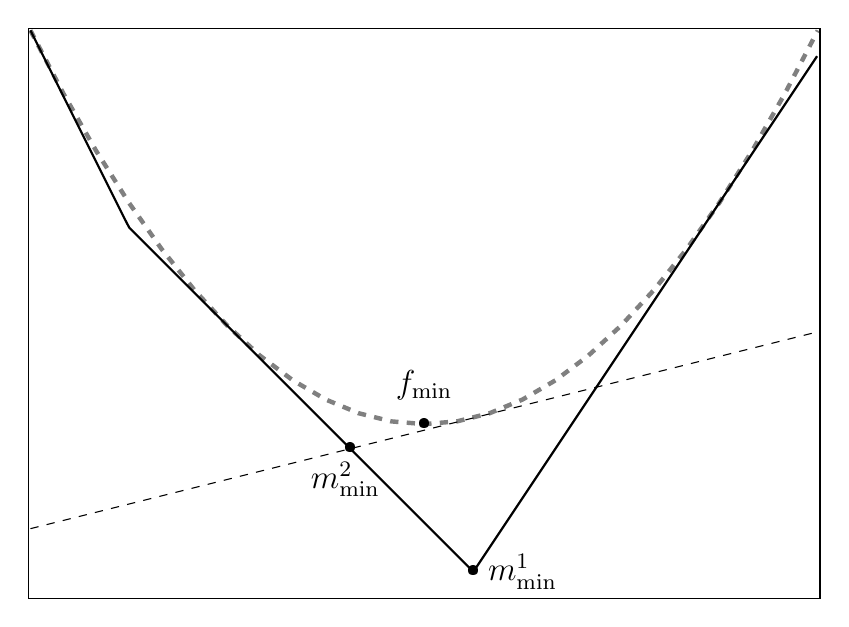
\begin{tikzpicture}[xscale=5,yscale=10]
\draw [gray,ultra thick,dashed,domain=0:2] plot (\x, {0.5*(\x-1)^2});
%\draw [dashed,domain=0:1] plot (\x, {-1*\x + 0.5});
%\draw [dashed,domain=0:2] plot (\x, {-\x/2 + 3/8});
%\draw [dashed,domain=1:2] plot (\x, {(3/4)*\x-1.03125});
\draw [thick,domain=0:2,samples=200] plot (\x, {max(-1*\x + 0.5,max(-\x/2 + 3/8,(3/4)*\x-1.03125))});
\node () at (1,0) {\textbullet};
\node [font=\large] () at (1,0.05) {$f_\text{min}$};
\node () at (1.125,-0.1875) {\textbullet};
\node [font=\large] () at (1.25,-0.1875) {$m_\text{min}^1$};
\draw [dashed,domain=0:2] plot (\x, {0.125*\x - 0.132813});
\node () at (0.812501,-0.0312504) {\textbullet};
\node [font=\large] () at (0.8,-0.07) {$m_\text{min}^2$};
\draw (current bounding box.north east) rectangle (current bounding box.south west);
\end{tikzpicture}
\caption{An iteration of the cutting-plane algorithm applied to $f = x^2$ ($n = 1$). The point $m_\text{min}^1$ is the minimizer of the current model. We then re-evaluate $f$ and add a \textit{cut} (dashed line) to the model corresponding to the new (sub)derivative. The point $m_\text{min}^2$ minimizes the new model. The point $f_\text{min}$ is the true minimizer.}\label{fig:cut}
\end{figure}
\begin{algorithm}
\caption{Cuting plane algorithm -- Serial}\label{algserial}
\begin{algorithmic}[1]
\REQUIRE Subdifferentiable functions $f_1,\ldots,f_n$. Starting point $x^1$.
\STATE $k \leftarrow 1$
\REPEAT
\FOR{$i=1$ \TO $n$}
\STATE Compute function value and subderivative $(f_i(x^k),g_{i,x^k})$ at $x^k$.
\ENDFOR
\STATE $x^{k+1} \leftarrow \operatorname{argmin}_x \sum_{i=1}^n m^k_i(x)$, with $m^k_i(x)$ defined by \eqref{eq:mod}
\STATE $k \leftarrow k + 1$
\UNTIL{convergence}
\end{algorithmic}
\end{algorithm}

An important observation is that the computation of the function values and subderivatives may be performed independently for each $i$ in the \textbf{for} loop. In many applications this computation is expensive, hence there is a real potential for speedup if we parallelize this loop. We will now investigate implementing and parallelizing this algorithm in Julia.

\section{Julia implementation}
In the previous section we presented the mathematical algorithm. Here we'll work with an actual implementation on a small toy problem and experiment with parallel computing in Julia. First, retrieve the code from \href{https://github.com/JuliaLang/IAP2013/tree/master/NumericalOptimization}{here}.
The \texttt{Tutorial.jl} file contains the code we will be referring to, while \texttt{ExampleSolution.jl} contains potential solutions to some of the exercises.

Our toy problem will be based on the functions $f_i(x) = \frac{1}{2}(x-i)^2$. With $f(x) = \sum_{i=1}^n f_i(x)$ as before, we have $f'(x) = \sum_{i=1}^n (x-i)$. Using basic calculus, we know already that the minimizer of $f$ is at $x = \frac{1}{n}\sum_{i=1}^n i = (n+1)/2$. Before running, install the Optim package, \texttt{Pkg.add("Optim")}. We can now run the the code by \texttt{julia Tutorial.jl}. The output should appear as follows:
\begin{center}
\begin{SaveVerbatim}{verb2}
Solving model with n = 10, initial solution: [0.5]
Optimal solutuon should be 5.5
Model minimizer: [10.0]
Model minimizer: [5.25]
Model minimizer: [7.625]
...
Model minimizer: [5.49995]
Converged in 15 iterations
elapsed time: 78.94296097755432 seconds
\end{SaveVerbatim}
\fbox{\BUseVerbatim{verb2}}
\end{center}

Let's open up the code. The function \texttt{f} implements the black-box calculation of the subderivatives. Notice the line with \texttt{sleep}, which we use to simulate a variably expensive black-box. The \texttt{evalmodel} function evaluates $\sum_{i=1}^n m_i^k(x)$ at \texttt{x} given the stored \texttt{subderivatives}. 

The \texttt{cpserial} function implements Algorithm~\ref{algserial} in serial. The parameter $N$ is our cursive $n$. The line \texttt{results = map(f,[(cur[1],i) for i in 1:N])} corresponds to loop of lines 3--5 of the algorithm. The call to \texttt{Optim.optimize} corresponds to line 6. Now for the fun stuff.

\begin{ex}
Insert code to plot $\sum_{i=1}^n m_i^k(x)$ versus $\sum_{i=1}^n f_i(x)$ at each iteration. You may use \href{https://github.com/nolta/Winston.jl}{Winston} or any other package.
\end{ex}

\begin{ex}
Review the Julia documentation on \href{http://docs.julialang.org/en/latest/manual/parallel-computing/}{parallel computing}. Modify the code so that the subderivatives are computed in parallel. \textit{(Hint: it only requires a small change.)}
\end{ex}

Now try running \texttt{julia -p 2 Tutorial.jl}. If you get an error like
\begin{center}
\begin{BVerbatim}
From worker 2:	exception on 2: f not defined
\end{BVerbatim}
\end{center}
this means that \texttt{f} was only defined on process 1, but you're trying to call it on process 2. Check the documentation or \texttt{ExampleSolution.jl} for a fix.

\begin{ex}\label{ex:par}
Change $n$ to 20 and run \texttt{julia -p nproc Tutorial.jl} for nproc = 1, 2, 3, 5, 10 on a machine with sufficiently many cores. Because of the explicit randomness in computing times, you may want to repeat and take average execution times. Do you observe speedup? Compute the parallel efficiency (observed speedup divided by perfect speedup) from 1 to 10 processes. 
\end{ex}

\begin{ex}
With \texttt{nproc} $= 1$, record and print out the total time spent in the \textit{serial bottleneck} of calling \texttt{Optim.optimize}. Use \href{http://en.wikipedia.org/wiki/Amdahl's\_law}{Amdahl's law} to compute the theoretical maximum possible speedup. Was this achieved in the previous exercise?
\end{ex}

\begin{advex}
Replace \texttt{Optim.optimize} with a faster approach for minimizing the model function. Hint: this problem can be solved efficiently by using Linear Programming. \textit{(Note: you should complete the rest of the tutorial before attempting this.)}
\end{advex}

\begin{ex}
Change the random \texttt{sleep} time inside \texttt{f} to a deterministic time, say 0.6 seconds. Repeat Exercise~\ref{ex:par}. Does the parallel efficiency change?
\end{ex}

You should have observed that the imbalance in computation time does have a significant effect on the parallel speedups observed. Let's visualize this effect. 

\begin{ex}
Modify the code so that each process records the intervals during which it spends inside the function \texttt{f}. Plot these intervals in some reasonable form, using Figure \ref{fig:act} as an example (source code in \texttt{ExampleSolution.jl}). This figure could be improved by plotting the time spent inside \texttt{Optim.optimize} as well. 
\end{ex}


\begin{figure}[ht]
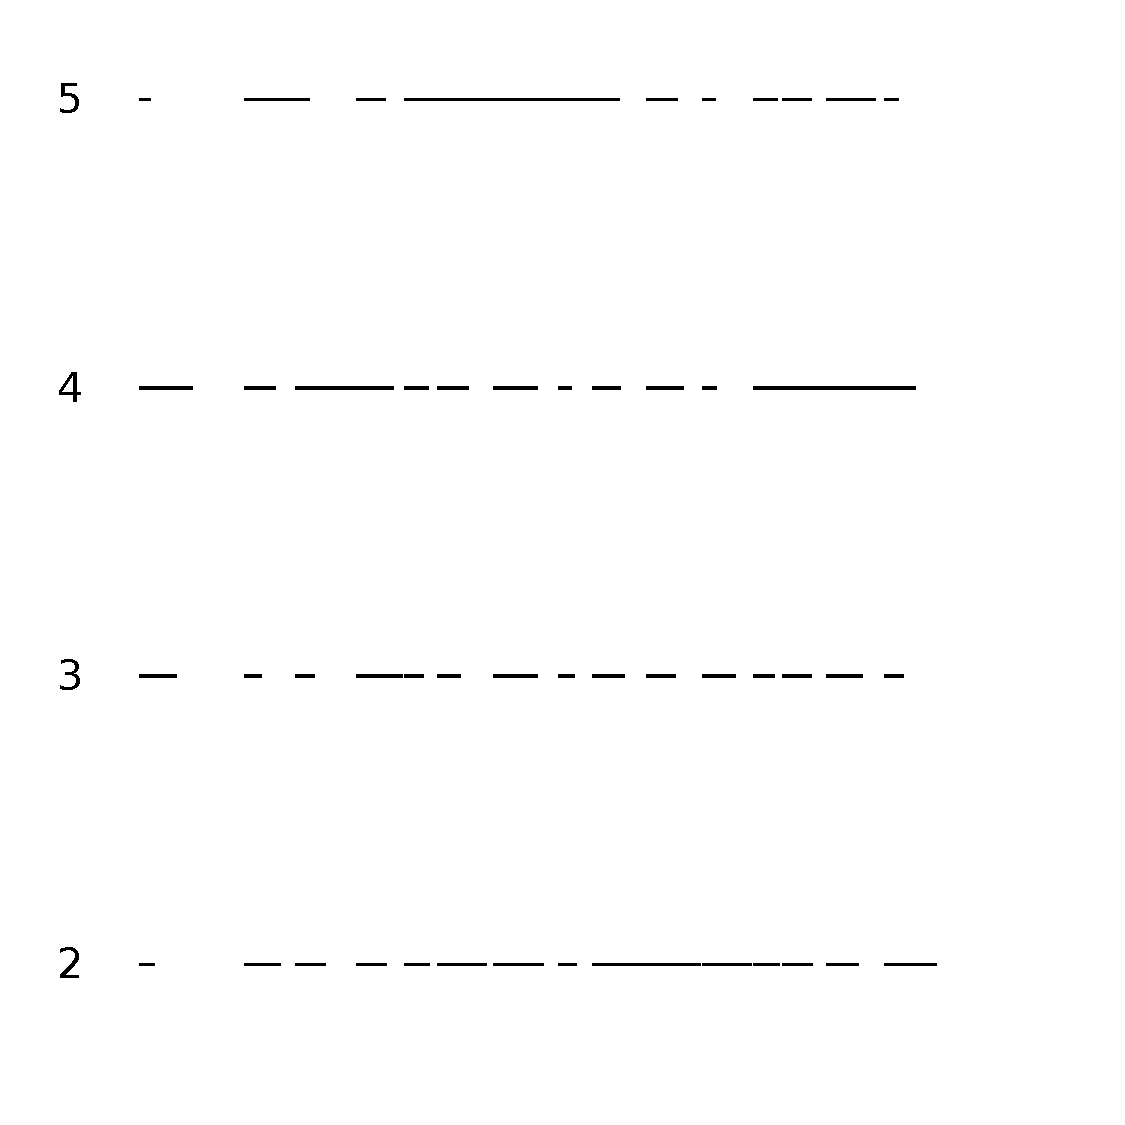
\includegraphics[scale=0.4]{activityplotnorm}
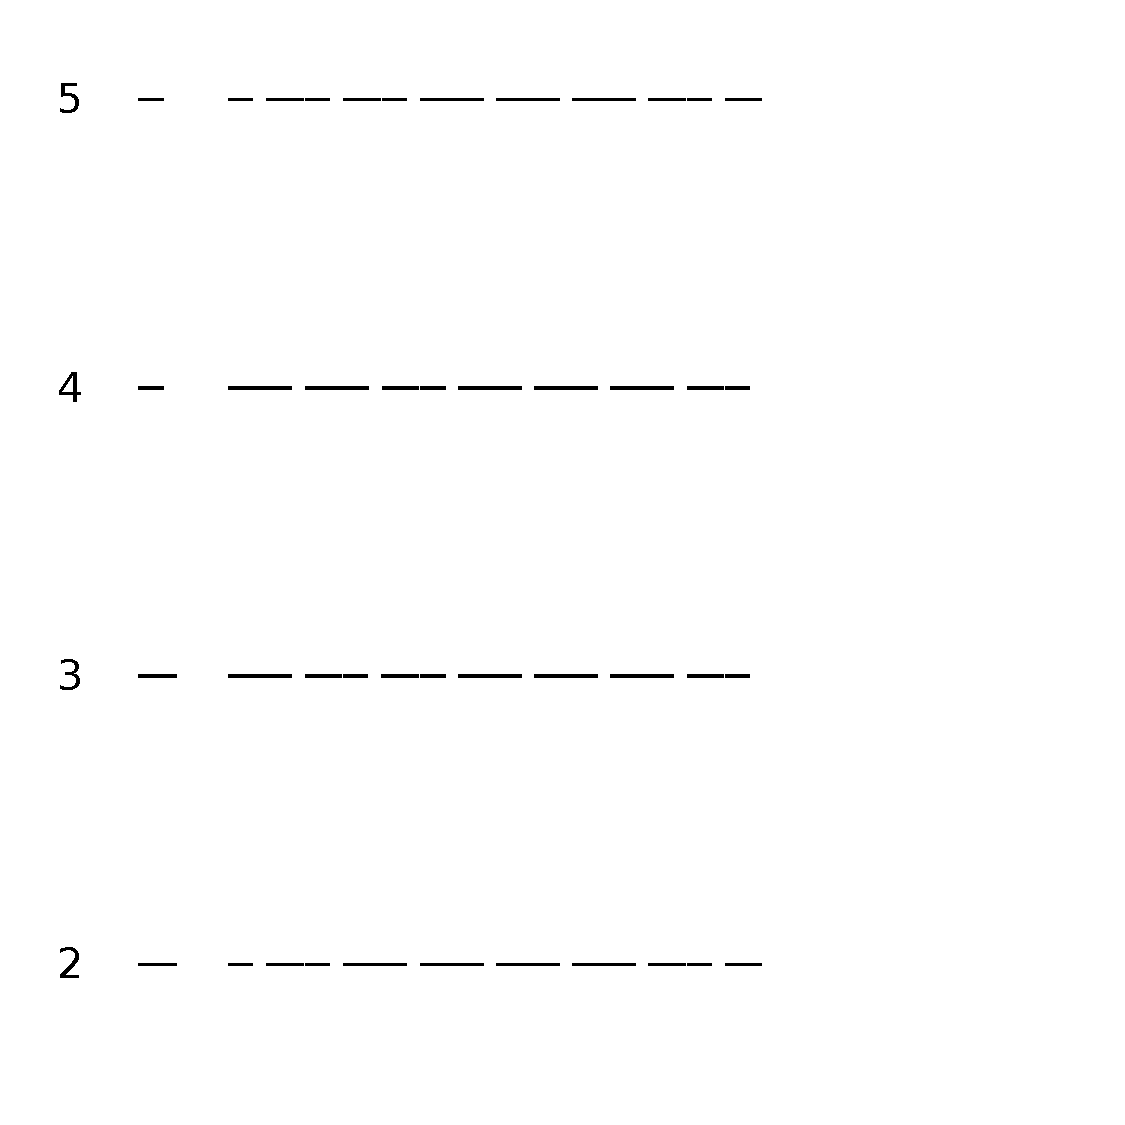
\includegraphics[scale=0.4]{activityplotdeterm}
\caption{Plots of process activity over time running on 5 processes (4 worker processes). Variable subproblem evaluation time on left, deterministic on right.  Black lines denote intervals of activity, white space indicates inactivity. }\label{fig:act}
\end{figure}

\begin{optex}
Try using \texttt{Base.pmap\_static} (take a look at its definition in \texttt{julia/base/multi.jl}). How does this affect performance and the previous discussion?
\end{optex}

\section{Asynchronous algorithm}
The asynchronous variant of the cutting-plane algorithm aims to reduce the idle time of the worker processes by eliminating the bottleneck of resolving the model. While previously the parallelism was hidden by high-level Julia functions, now we will need to explicitly consider the master process and the set of workers.

The idea of the asynchronous algorithm is to minimize the model function using \textit{incomplete information} in order to generate new tasks to feed to workers. That is, instead of waiting for all subderivatives to be computed at a given candidate solution, we generate a new candidate solution (and a full set of new subgradient evaluation tasks) once some proportion $\sigma$ of the subderivatives have been computed. These tasks may be immediately fed to workers, hence workers will spend less time waiting for new tasks. Further description is beyond the scope of this tutorial; see \cite{Linderoth03}.

The asynchronous algorithm is implemented as \texttt{asyncversion} in \texttt{Tutorial.jl}. It is worth spending a few minutes trying to understand the code. The use of \href{http://docs.julialang.org/en/latest/manual/control-flow/#man-tasks}{Julia tasks} with \texttt{@spawnlocal} and \texttt{@sync} is not intuitively obvious (at least to me). As a starting point, compare with the implementation of \texttt{pmap} in \texttt{julia/base/multi.jl}.

\begin{ex}
Run both the original parallel code and the asynchronous code with $n = 100$ and nprocs $= 5, 10, 20$, under the original random computation time model (\texttt{max(0.1,0.2+1*randn())}). Is the asynchronous code faster? Note that because less information is used to generate the iterates, the asynchronous version typically requires more iterations. Compare both the total execution time and the average rate of subproblems solved per second.
\end{ex}

\begin{ex}
Experiment with different random models for computation time. What happens if you increase or decrease the variance (the coefficient of \texttt{randn()})?
\end{ex}

\begin{advex}
Currently \texttt{Optim.optimize} is called by the same process that manages the workers. Modify the code so that new tasks can be distributed in the middle of calls to \texttt{Optim.optimize}.
\end{advex}


\bibliography{refs}{}
\bibliographystyle{plain}

\end{document}